\section{DA Wandler\hartl{455}}
  Es gibt 3 Verfahren: Parallelverfahren, Wägeverfahren und Zählverfahren.
\subsection{Wägeverfahren\hartl{461}} 
\begin{longtable}{|p{3cm}|c|p{8.6cm}|}
	\hline
	\textbf{Spannungs"-summierung \hartl{461}}
	& \includegraphics[width=3.5cm, valign=t]{./images/spannungssummierung.png}
	& {\begin{align*}
		V_{Out} &= \frac{B0\cdot 2^0 + B1 \cdot 2^1+ \ldots + B(n-1)\cdot 2^{n-1}}{2^n} \\
    & \cdot (V_{Refp}-V_{Refn}) + V_{Refn}
	  \end{align*}}
    
	  \begin{description}
  		\item[Vorteile:] n Widerstände, n Schalter
  		\item[Nachteile:] nicht garantiert stetig, grosse Wertebereiche für Widerstände, rechnen mit Leitwerten ($G_0 = \frac{1}{8R}$)
	  \end{description}
	\\ \hline
	\textbf{Wägeverfahren mit Ausgangstreiber} \newline
  (Summation gewichteter Ströme)
	& \includegraphics[width=5cm, valign=t]{./images/praktisch.png}
	& \[ Idac_{max}=\frac{V_{Refp}-V_{Refn}}{R} \cdot \frac{2^n-1}{2^n} \] \newline
    Vout und Idac\_inv sind differentiell zueinander, dadurch fliesst immer der gleiche Strom
    und der Offsetfehler bleibt konstant.
	\\ \hline
	\textbf{R-2R-Netzwerk \hartl{462}} Multiplizierende Wandler wandeln die Referenzspannung in Ströme um.
	& \includegraphics[width=5.5cm, valign=t]{./images/r2rnetzwerk.png}
	& {
	\begin{align*}
		V_{out,max} &= V_{Refn} \\
		V_{out,min} &= V_{Refn} - R \cdot I_{max}\\
		I_{max}		&= (V_{Refp} - V_{Refn}) (\frac{1}{2R} + \frac{1}{2}\frac{1}{2R} + \frac{1}{4} \frac{1}{2R} + \ldots) \\
					&= (V_{Refp} - V_{Refn})\frac{1}{2R}(2-2^{1-n})
	\end{align*}}
  
  \begin{description}
    \item[Vorteil:] nur 2 unterschiedliche R
    \item[Nachteil:] es muss immer ein Strom fliessen
  \end{description}
  
	\\ \hline
	\textbf{R-2R-Netzwerk}
	& \includegraphics[width=5cm, valign=t]{images/r2r.png}
	& {
	\begin{align*}
		V_{out}&= \frac{V_{ref}}{2^n} + \frac{R_L}{R_L + R} \cdot D
	\end{align*}}
  
	\\ \hline
	\textbf{Kapazitiver DAC (Charge Scaling)}
	& \includegraphics[width=6cm, valign=t]{./images/kapazitiverDAC.png}
	& { \textbf{ Vorteil:} Man kann bis zur angelegten Referenzspannung durchschalten \newline
        \begin{align*}
		C1	&= B3 \cdot 8C+B2 \cdot 4C+ B1 \cdot 2C+B0 \cdot C \\
		C2	&= !B3 \cdot 8C+!B2 \cdot 4C+ !B1 \cdot 2C+!B0 \cdot C+C \\
		V_{Out}& =\frac{C1}{C1+C2}\cdot (V_{Rp}-V_{Rn}) + V_{Rn} \textrm{mit } C1+C2=2^n\cdot C\\
		V_{out} &= \frac{D}{2^n} \cdot \left(V_{rp}-{V_{Rn}}\right) + V_{Rn}
	  \end{align*}}
	\\ \hline
    \textbf{Kapazitiver DAC mit Ausgangstreiber}
    & \includegraphics[width=6cm, valign=t]{./images/kapazitiverDACmitAmp.png}
    & {Wenn z.B. B3 auf $V_{Ref1}$ geschaltet wird:\newline
      \begin{align*}
          Q_{C3} &= C_3 \cdot \Delta U = C_3 \cdot (V_{Ref1}-V_{Ref2})\\
          \Delta Q_3 &= \Delta Q_{fb} = C_3 \cdot \Delta V_{Ref}\\
          &\Rightarrow \Delta V_{Out} = \frac{\Delta Q_{fb}}{C_{fb}} = (V_{Ref1}-V_{Ref2}) \cdot \frac{C_3}{C_{fb}} \\
          V_{out} &= V_{Ref2}-\Delta V_{Out} 
      \end{align*}}
    \\ \hline
\end{longtable}

\subsection{Zählverfahren (PWM)\hartl{466}}
\begin{longtable}{|>{\bfseries}p{4cm}|l|p{8cm}|}
	\hline 
	Grundprinzip \hartl{466}
	& \includegraphics[width=6cm, valign=t]{./images/pwm_DAC.png}
	& $ V_{Out}=\frac{D}{2^n} \cdot (V_{Refp}-V_{Refn})+V_{Refn} $ \newline
	\begin{tabular}{lp{5cm}}
    \textbf{Vorteile:} 
      &-einfache Schaltung \\
      &-ermöglicht hohe Auflösung \\
      &-Funktioniert ohne analoge Schaltungen on Chip \\
    
    \textbf{Nachteile:}
      &-sehr langsam \\
      &-benötigt grosse Zeitkonstanten 
  \end{tabular}
	\\ \hline
	PWM-Ansteuerung \hartl{466}
	& \parbox[c][2cm]{6cm}{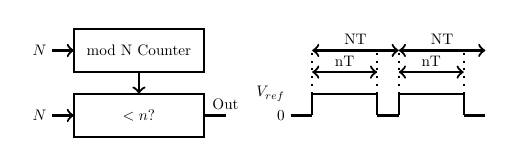
\begin{tikzpicture}[thick, transform shape, scale=0.55]
	\draw node at (0.5,0) [anchor=east] {$N$};
	\draw [->] (0.5,0) -- (1,0);
	\draw (1,0.5) rectangle (4,-0.5);
	\draw node at (2.5,0) {mod N Counter};
	
	\draw [->] (2.5,-0.5) -- (2.5,-1);
	
	\draw node at (0.5,-1.5) [anchor=east] {$N$};
	\draw [->] (0.5,-1.5) -- (1,-1.5);
	\draw (1,-1) rectangle (4,-2);
	\draw node at (2.5,-1.5) {$<n?$};
	
	\draw (4,-1.5) -- (4.5,-1.5) node [anchor=south] {Out};
	
	%PWM Signal:
	\node at (6,-1) [anchor=east] {$V_{ref}$};
	\node at (6,-1.5) [anchor=east] {$0$};
	
	\foreach \x in {6.5,8,8.5,10}
	{
		\draw (\x,-1) -- (\x,-1.5);
		\draw [dotted] (\x,-1) -- (\x,0);
	}
	\foreach \x in {6,8,10}
		\draw (\x,-1.5) -- (\x+0.5,-1.5);
	\foreach \x in {6.5,8.5}
		\draw (\x,-1) -- (\x+1.5,-1);
	
	\foreach \x in {6.5,8.5}
	{
		\draw [<->] (\x,0) -- (\x+2,0);
		\node at (\x+1,0) [anchor=south] {NT};
	}
	\foreach \x in {6.5,8.5}
	{
		\draw [<->] (\x,-0.5) -- (\x+1.5,-0.5);
		\node at (\x+0.75,-0.5) [anchor=south] {nT};
	}

\end{tikzpicture}}
	& $\bar{V_{Out}}=\frac{n}{N}V_{Ref}$
	  \begin{tabular}{ll}
		N:&Takte\\
		n:&digitale Eingangsgrösse
	  \end{tabular}
	\\ \hline
\end{longtable}

\subsection{Parallelverfahren}
\renewcommand{\arraystretch}{1}
\begin{longtable}{|>{\bfseries}p{3cm}|c|p{7.6cm}|}
	\hline
	Strom-DAC\hartl{456}  
	& \raisebox{-.2\totalheight}{\includegraphics[width=7cm, valign=t]{images/Strom-DAC}}
	& {\begin{align*}
      K &=2^N-1 \qquad I_{out} = D \cdot I = D \cdot \frac{V_{Ref}}{R}\\
      I &=\frac{V_{Ref}}{R} \qquad \text{(von einer Quelle)}
	  \end{align*}}
	  
	  \begin{tabular}{lp{5.8cm}}
	  	K: & Anz. Stromquellen \\
      D: & Eingangswert (Anz. aktive Schalter) \\
      \multicolumn{2}{l}{Schaltereigenschaften:}\\
      On: & kein Spannungsabfall  \\
      Off: & kein Strom
    \end{tabular} 
    \begin{description}
  		\item[Vorteile: ] Schnell (Stromgesteuert)
  		\item[Nachteile:] 
	  \end{description} 
	\\ \hline
	String DAC (Voltage Scaling) \hartl{459}
	& \raisebox{-.1\totalheight}{\includegraphics[width=5.5cm, valign=t]{images/string_DAC}}
	& 
		\begin{description}
  		\item[Vorteile: ] garantierte Stetigkeit
  		\item[Nachteile:] benötigt $2^n$ Widerstände und $2^n$ Schalter, n-to-$2^n$ Decoder(linke Variante),
        er darf nicht belastet werden und hat grossen Schaltungsaufwand.
	  \end{description} 
    
	  {\begin{align*}
	  	V_{Out_{ideal}}(D) = \frac{D}{2^n}(V_{Refp}-V_{Refn})+V_{Refn}\\
	  	V_{Out_{real}}(D) = V_{Refn}+\left(V_{Refp}-V_{Refn}\right)\cdot\\
	  		\cdot\frac{D \cdot R_{Load}}{2^n \cdot R \cdot D-R \cdot D^2 + 2^n (R_{Load} + R_{Switch}) }\\
	  	DAC_{error}(D)=\frac{V_{Out_{real}}(D)-V_{Out_{ideal}}(D)}{V_{Out_{ideal}}(D)}
	  \end{align*}}
	  
	\\ \hline
	Segmented String DAC \hartl{459}
	& \raisebox{-.1\totalheight}{\includegraphics[width=5.6cm, height = 4cm, valign=t]{images/segmented_string_DAC}}
	& \begin{description}
  		\item[Vorteile: ] viel weniger Elemente
  		\item[Nachteile:] benötigt Buffer (offset-frei)
	  \end{description}
	\\ \hline
\end{longtable}
\renewcommand{\arraystretch}{\arraystretchOriginal}


%\newpage



\subsection{Weitere DAC}
\begin{longtable}{|>{\bfseries}p{4cm}|c|p{8cm}|}
	\hline
	Kaskadierte DAC
	& \includegraphics[width=5cm, valign=t]{./images/kaskadiertDAC.png}
	& \begin{itemize}
  		\item MS-DAC hat 2 Ausgangsspannungen (Über und unter gewünschtem
  			$V_{Out}$)
  		\item LS-DAC hat kleine Eingangsspannungsdifferenz $\to$ höhere Auflösung der Spannung
	  \end{itemize}
	\\ \hline
	Zyklisch, algorithmischer DAC \hartl{466}
	& \includegraphics[width=6cm, valign=t]{./images/zyklischDAC.png}
	& \textbf{Ablauf der Wandlung}
	  \begin{enumerate}
  		\item Spg. im S/H löschen (Schalter S1), S3 offen
  		\item S1 auf den Verstärker-Ausgang schalten
  		\item Laufvariale k wird auf 0 gesetzt
  		\item S2 setzen: VREF oder GND ( abh. $D_{K}$).
  		\item Addierer und Verstärker generieren Ausgangssignal
  		\item Im S/H wird Feedback-Spannung gespeichert (S1)
  		\item X wird um 1 erhöht
  		\item Gehe zu Schritt 4, wenn $X\leq n$
	  \end{enumerate}
	\\ \hline
	Pipelined DAC 
	& \includegraphics[width=6cm, valign=t]{images/pipelinedDAC}
	& $V_{Out} = (D_0 \cdot 2^{-n} + D_1 \cdot 2^{1-n} + ... + D_{n-1} \cdot 2^{-1})\cdot V_{Ref}$\newline\newline
      Die Latenz beträgt n Zyklen, die Update-Frequenz ist aber n-mal grösser, da die Blöcke n-fach vorliegen.\newline
      LSB ($\mathrm{D_0}$): $\mathrm{V_{Ref}}$ wird n-mal halbiert
	\\ \hline
	Strom-DAC
	& \includegraphics[width=6cm, valign=t]{images/stromDAC}
	& \begin{itemize}
  		\item Stromspiegel
  		\item MP0 ist gleich breit wie Stromquellen-MOS $\to \mathrm{I(MP0)=I_{Ref}} \qquad$ MP0: Einheitstransistor
  		\item MP1 ist doppelt so breit wie MP0 $\to \mathrm{I(MP1)}=2*\mathrm{I_{Ref}} \qquad$ MP1: 2 Einheitstransistoren
  		\item MP2 ist doppelt so breit wie MP1 $\to \mathrm{I(MP2)}=4*\mathrm{I_{Ref}} \qquad$ MP2: 4 Einheitstransistoren
  		\item \ldots
	  \end{itemize}
	\\ \hline
\end{longtable}

\subsection{Spezielle Wandler}
\begin{longtable}{|>{\bfseries}p{4cm}|c|p{8cm}|}
  \hline
    Digitales Potentiometer \hartl{460}
    & \includegraphics[width=5cm, valign=t]{images/digitales_potentiometer}
    & \begin{itemize}
        \item automatisierter Elektronik-Test möglich
        \item D (digitale Wert) wird im PROM gespeichert
        \item V(A), V(B) können variabel sein
      \end{itemize} \\
%  \hline
%    Multiplizierende Wandler
%    & 
%    & Wandler bei denen mit Widerständen aus der Referenzspannung Ströme abgeleitet werden.
%    z.B R2R-Netzwerk \\
  \hline
    DAC mit Exponentieller Funktion
    &\includegraphics[width=6cm, valign=t]{images/DAC_exp.png}
    & \\
  \hline
\end{longtable}

\subsection{Ausgangsverstärker}
\begin{minipage}{7cm}
	\includegraphics[width=6.5cm]{images/Ausgangsverstaerker.png}
\end{minipage}
\begin{minipage}{12cm}
  $C_{Filter}$ dämpft Glitches beim Umschalten des Digitalwertes.
  \begin{align*}
  	V_{opp} &= 0V \hdots I_{OUT} \cdot (25\Omega || 1.5k\Omega) \\
  	V_{opn} &= 0V \hdots \overline{I_{OUT}} \cdot (25\Omega || 1.5k\Omega) \cdot \frac{1k\Omega}{1.5k\Omega} = V_{opp} \cdot \frac{1k\Omega}{1.5k\Omega} \\
  	A_{pos} &= 1 + \frac{1k\Omega}{500\Omega + 25\Omega}
  \end{align*}
\end{minipage}

